\documentclass[tikz]{standalone}

\begin{document}

\tikzset{every picture/.style={line width=0.75pt}} %set default line width to 0.75pt        

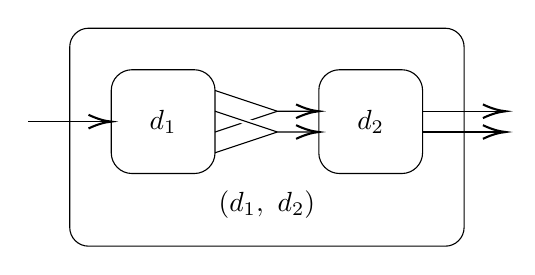
\begin{tikzpicture}[x=0.75pt,y=0.75pt,yscale=-1,xscale=1]
  %uncomment if require: \path (0,150); %set diagram left start at 0, and has height of 150

  %Straight Lines [id:da4656163938598641] 
  \draw  (100,80) -- (130,70) ;
  %Straight Lines [id:da010224775030959865] 
  \draw [color={rgb, 255:red, 254; green, 254; blue, 254 }  ,draw opacity=1 ][line width=2.25]	(100,70) -- (130,80) ;
  %Rounded Rect [id:dp45414365465445616] 
  \draw (150,60) .. controls (150,54.48) and (154.48,50) .. (160,50) -- (190,50) .. controls (195.52,50) and
  (200,54.48) .. (200,60) -- (200,90) .. controls (200,95.52) and (195.52,100) .. (190,100) -- (160,100) .. controls
  (154.48,100) and (150,95.52) .. (150,90) -- cycle ;
  %Rounded Rect [id:dp651922272663219] 
  \draw (50,60) .. controls (50,54.48) and (54.48,50) .. (60,50) -- (90,50) .. controls (95.52,50) and (100,54.48) ..
  (100,60) -- (100,90) .. controls (100,95.52) and (95.52,100) .. (90,100) -- (60,100) .. controls (54.48,100) and
  (50,95.52) .. (50,90) -- cycle ;
  %Rounded Rect [id:dp9191842348834878] 
  \draw (30,39.04) .. controls (30,34.05) and (34.05,30) .. (39.04,30) -- (210.96,30) .. controls (215.95,30) and
  (220,34.05) .. (220,39.04) -- (220,125.96) .. controls (220,130.95) and (215.95,135) .. (210.96,135) -- (39.04,135)
  ..
  controls (34.05,135) and (30,130.95) .. (30,125.96) -- cycle ;
  %Straight Lines [id:da9548799664934018] 
  \draw  (100,60) -- (130,70) -- (148,70) ;
  \draw [shift={(150,70)}, rotate = 180] [color={rgb, 255:red, 0; green, 0; blue, 0 }  ][line width=0.75]
  (10.93,-3.29) .. controls (6.95,-1.4) and (3.31,-0.3) .. (0,0) .. controls (3.31,0.3) and (6.95,1.4) .. (10.93,3.29)
  ;
  %Straight Lines [id:da8489089431604431] 
  \draw  (100,70) -- (130,80) ;
  %Straight Lines [id:da7337117296199642] 
  \draw  (100,90) -- (130,80) -- (148,80) ;
  \draw [shift={(150,80)}, rotate = 180] [color={rgb, 255:red, 0; green, 0; blue, 0 }  ][line width=0.75]
  (10.93,-3.29) .. controls (6.95,-1.4) and (3.31,-0.3) .. (0,0) .. controls (3.31,0.3) and (6.95,1.4) .. (10.93,3.29)
  ;
  %Straight Lines [id:da7108546306775476] 
  \draw  (10,75) -- (48,75) ;
  \draw [shift={(50,75)}, rotate = 180] [color={rgb, 255:red, 0; green, 0; blue, 0 }  ][line width=0.75]
  (10.93,-3.29)
  .. controls (6.95,-1.4) and (3.31,-0.3) .. (0,0) .. controls (3.31,0.3) and (6.95,1.4) .. (10.93,3.29)	 ;
  %Straight Lines [id:da24088993087372645] 
  \draw  (200,70) -- (238,70) ;
  \draw [shift={(240,70)}, rotate = 180] [color={rgb, 255:red, 0; green, 0; blue, 0 }  ][line width=0.75]
  (10.93,-3.29) .. controls (6.95,-1.4) and (3.31,-0.3) .. (0,0) .. controls (3.31,0.3) and (6.95,1.4) .. (10.93,3.29)
  ;
  %Straight Lines [id:da5401552925318207] 
  \draw  (200,80) -- (238,80) ;
  \draw [shift={(240,80)}, rotate = 180] [color={rgb, 255:red, 0; green, 0; blue, 0 }  ][line width=0.75]
  (10.93,-3.29) .. controls (6.95,-1.4) and (3.31,-0.3) .. (0,0) .. controls (3.31,0.3) and (6.95,1.4) .. (10.93,3.29)
  ;

  % Text Node
  \draw (125,115) node	 [align=left] {$\displaystyle \Merge( d_{1} ,\ d_{2})$};
  % Text Node
  \draw (75,75) node   [align=left] {$\displaystyle d_{1}$};
  % Text Node
  \draw (175,75) node	[align=left] {$\displaystyle d_{2}$};

\end{tikzpicture}
\end{document}
